\chapter{Бэкап и восстановление PostgreSQL}

\begin{epigraphs}
\qitem{Есть два типа администраторов~--- те, кто не делает бэкапы, и те, кто уже делает}{Народная мудрость}
\qitem{Если какая-нибудь неприятность может произойти, она случается}{Закон Мэрфи}
\end{epigraphs}

\section{Введение}

Любой хороший сисадмин знает~--- бэкапы нужны всегда. Насколько бы надежной ни казалась Ваша система, всегда может произойти случай, который был не учтен, и из-за которого могут быть потеряны данные.

Тоже самое касается и PostgreSQL баз данных. Посыпавшийся винчестер на сервере, ошибка в файловой системе, ошибка в другой программе, которая перетерла весь каталог PostgreSQL и многое другое приведет только к плачевному результату. И даже если у Вас репликация с множеством слейвов, это не означает, что система в безопасности~--- неверный запрос на мастер (\lstinline!DELETE/DROP/TRUNCATE!), и у слейвов такая же порция данных (точнее их отсутствие).

Существуют три принципиально различных подхода к резервному копированию данных PostgreSQL:

\begin{itemize}
  \item SQL бэкап;
  \item Бэкап уровня файловой системы;
  \item Непрерывное резервное копирование;
\end{itemize}

Каждый из этих подходов имеет свои сильные и слабые стороны.


\section{SQL бэкап}

Идея этого подхода в создании текстового файла с командами SQL. Такой файл можно передать обратно на сервер и воссоздать базу данных в том же состоянии, в котором она была во время бэкапа. У PostgreSQL для этого есть специальная утилита~--- \lstinline!pg_dump!. Пример использования \lstinline!pg_dump!:

\begin{lstlisting}[language=Bash,label=lst:backups1,caption=Создаем бэкап с помощью pg\_dump]
$ pg_dump dbname > outfile
\end{lstlisting}

Для восстановления такого бэкапа достаточно выполнить:

\begin{lstlisting}[language=Bash,label=lst:backups2,caption=Восстанавливаем бэкап]
$ psql dbname < infile
\end{lstlisting}

При этом базу данных \lstinline!dbname! потребуется создать перед восстановлением. Также потребуется создать пользователей, которые имеют доступ к данным, которые восстанавливаются (это можно и не делать, но тогда просто в выводе восстановления будут ошибки). Если нам требуется, чтобы восстановление прекратилось при возникновении ошибки, тогда потребуется восстанавливать бэкап таким способом:

\begin{lstlisting}[language=Bash,label=lst:backups3,caption=Восстанавливаем бэкап]
$ psql --set ON_ERROR_STOP=on dbname < infile
\end{lstlisting}

Также, можно делать бэкап и сразу восстанавливать его в другую базу:

\begin{lstlisting}[language=Bash,label=lst:backups4,caption=Бэкап в другую БД]
$ pg_dump -h host1 dbname | psql -h host2 dbname
\end{lstlisting}

После восстановления бэкапа желательно запустить \lstinline!ANALYZE!, чтобы оптимизатор запросов обновил статистику.

А что, если нужно сделать бэкап не одной базы данных, а всех, да и еще получить в бэкапе информацию про роли и таблицы? В таком случае у PostgreSQL есть утилита \lstinline!pg_dumpall!. \lstinline!pg_dumpall! используется для создания бэкапа данных всего кластера PostgreSQL:

\begin{lstlisting}[language=Bash,label=lst:backups5,caption=Бэкап кластера PostgreSQL]
$ pg_dumpall > outfile
\end{lstlisting}

Для восстановления такого бэкапа достаточно выполнить от суперпользователя:

\begin{lstlisting}[language=Bash,label=lst:backups6,caption=Восстановления бэкапа PostgreSQL]
$ psql -f infile postgres
\end{lstlisting}


\subsection{SQL бэкап больших баз данных}

Некоторые операционные системы имеют ограничения на максимальный размер файла, что может вызывать проблемы при создании больших бэкапов через \lstinline!pg_dump!. К счастью, \lstinline!pg_dump! можете бэкапить в стандартный вывод. Так что можно использовать стандартные инструменты Unix, чтобы обойти эту проблему. Есть несколько возможных способов:

\begin{itemize}
  \item \textbf{Использовать сжатие для бэкапа}

Можно использовать программу сжатия данных, например GZIP:

\begin{lstlisting}[language=Bash,label=lst:backups7,caption=Сжатие бэкапа PostgreSQL]
$ pg_dump dbname | gzip > filename.gz
\end{lstlisting}

Восстановление:

\begin{lstlisting}[language=Bash,label=lst:backups8,caption=Восстановление бэкапа PostgreSQL]
$ gunzip -c filename.gz | psql dbname
\end{lstlisting}

или

\begin{lstlisting}[language=Bash,label=lst:backups9,caption=Восстановление бэкапа PostgreSQL]
cat filename.gz | gunzip | psql dbname
\end{lstlisting}

\item \textbf{Использовать команду split}

Команда split позволяет разделить вывод в файлы меньшего размера, которые являются подходящими по размеру для файловой системы. Например, бэкап делится на куски по 1 мегабайту:

\begin{lstlisting}[language=Bash,label=lst:backups10,caption=Создание бэкапа PostgreSQL]
$ pg_dump dbname | split -b 1m - filename
\end{lstlisting}

Восстановление:

\begin{lstlisting}[language=Bash,label=lst:backups11,caption=Восстановление бэкапа PostgreSQL]
$ cat filename* | psql dbname
\end{lstlisting}

  \item \textbf{Использовать пользовательский формат дампа \lstinline!pg_dump!}

PostgreSQL построен на системе с библиотекой сжатия Zlib, поэтому пользовательский формат бэкапа будет в сжатом виде. Это похоже на метод с использованием GZIP, но он имеет дополнительное преимущество~--- таблицы могут быть восстановлены выборочно. Минус такого бэкапа~--- восстановить возможно только в такую же версию PostgreSQL (отличаться может только патч релиз, третья цифра после точки в версии):

\begin{lstlisting}[language=Bash,label=lst:backups12,caption=Создание бэкапа PostgreSQL]
$ pg_dump -Fc dbname > filename
\end{lstlisting}

Через psql такой бэкап не восстановить, но для этого есть утилита \lstinline!pg_restore!:

\begin{lstlisting}[language=Bash,label=lst:backups13,caption=Восстановление бэкапа PostgreSQL]
$ pg_restore -d dbname filename
\end{lstlisting}

\end{itemize}

При слишком большой базе данных, вариант с командой split нужно комбинировать со сжатием данных.



\section{Бэкап уровня файловой системы}

Альтернативный метод резервного копирования заключается в непосредственном копировании файлов, которые PostgreSQL использует для хранения данных в базе данных. Например:

\begin{lstlisting}[language=Bash,label=lst:backups14,caption=Бэкап PostgreSQL файлов]
$ tar -cf backup.tar /usr/local/pgsql/data
\end{lstlisting}

Но есть два ограничения, которые делает этот метод нецелесообразным, или, по крайней мере, уступающим SQL бэкапу:

\begin{itemize}
  \item PostgreSQL база данных должна быть остановлена, для того, чтобы получить актуальный бэкап (PostgreSQL держит множество объектов в памяти, буферизация файловой системы). Излишне говорить, что во время восстановления такого бэкапа потребуется также остановить PostgreSQL;
  \item Не получится восстановить только определенные данные с такого бэкапа;
\end{itemize}

Как альтернатива, можно делать снимки (snapshot) файлов системы (папки с файлами PostgreSQL). В таком случае останавливать PostgreSQL не требуется. Однако, резервная копия, созданная таким образом, сохраняет файлы базы данных в состоянии, как если бы сервер базы данных был неправильно остановлен. Поэтому при запуске PostgreSQL из резервной копии, он будет думать, что предыдущий экземпляр сервера вышел из строя и восстановит данные в соотвествии с данными журнала WAL. Это не проблема, просто надо знать про это (и не забыть включить WAL файлы в резервную копию). Также, если файловая система PostgreSQL распределена по разным файловым системам, то такой метод бэкапа будет очень ненадежным~--- снимки файлов системы должны быть сделаны одновременно. Почитайте документацию файловой системы очень внимательно, прежде чем доверять снимкам файлов системы в таких ситуациях.

Также возможен вариант с использованием \lstinline!rsync! утилиты. Первым запуском rsync мы копируем основные файлы с директории PostgreSQL (PostgreSQL при этом продолжает работу). После этого мы останавливаем PostgreSQL и запускаем повторно \lstinline!rsync!. Второй запуск \lstinline!rsync! пройдет гораздо быстрее, чем первый, потому что будет передавать относительно небольшой размер данных, и конечный результат будет соответствовать остановленной СУБД. Этот метод позволяет делать бэкап уровня файловой системы с минимальным временем простоя.


\section{Непрерывное резервное копирование}

PostgreSQL поддерживает упреждающую запись логов (Write Ahead Log, WAL) в \lstinline!pg_xlog! директорию, которая находится в директории данных СУБД. В логи пишутся все изменения, сделанные с данными в СУБД. Этот журнал существует прежде всего для безопасности во время краха PostgreSQL: если происходят сбои в системе, базы данных могут быть восстановлены с помощью <<перезапуска>> этого журнала. Тем не менее, существование журнала делает возможным использование третьей стратегии для резервного копирования баз данных: мы можем объединить бэкап уровня файловой системы с резервной копией WAL файлов. Если требуется восстановить такой бэкап, то мы восстанавливаем файлы резервной копии файловой системы, а затем <<перезапускаем>> с резервной копии файлов WAL для приведения системы к актуальному состоянию. Этот подход является более сложным для администрирования, чем любой из предыдущих подходов, но он имеет некоторые преимущества:

\begin{itemize}
  \item Не нужно согласовывать файлы резервной копии системы. Любая внутренняя противоречивость в резервной копии будет исправлена путем преобразования журнала (не отличается от того, что происходит во время восстановления после сбоя);
  \item Восстановление состояния сервера для определенного момента времени;
  \item Если мы постоянно будем <<скармливать>> файлы WAL на другую машину, которая была загружена с тех же файлов резервной базы, то у нас будет находящийся всегда в актуальном состоянии резервный сервер PostgreSQL (создание сервера горячего резерва);
\end{itemize}

Как и бэкап файловой системы, этот метод может поддерживать только восстановление всей базы данных кластера. Кроме того, он требует много места для хранения WAL файлов.

\subsection{Настройка}

Первый шаг~--- активировать архивирование. Эта процедура будет копировать WAL файлы в архивный каталог из стандартного каталога \lstinline!pg_xlog!. Это делается в файле \lstinline!postgresql.conf!:

\begin{lstlisting}[label=lst:backups15,caption=Настройка архивирования]
archive_mode = on # enable archiving
archive_command = 'cp -v %p /data/pgsql/archives/%f'
archive_timeout = 300 # timeout to close buffers
\end{lstlisting}

После этого необходимо перенести файлы (в порядке их появления) в архивный каталог. Для этого можно использовать функцию \lstinline!rsync!. Можно поставить функцию в \lstinline!cron! и, таким образом, файлы могут автоматически перемещаться между хостами каждые несколько минут:

\begin{lstlisting}[language=Bash,label=lst:backups16,caption=Копирование WAL файлов на другой хост]
$ rsync -avz --delete prod1:/data/pgsql/archives/ \
/data/pgsql/archives/ > /dev/null
\end{lstlisting}

В конце необходимо скопировать файлы в каталог \lstinline!pg_xlog! на сервере PostgreSQL (он должен быть в режиме восстановления). Для этого необходимо в каталоге данных PostgreSQL создать файл \lstinline!recovery.conf! с заданной командой копирования файлов из архива в нужную директорию:

\begin{lstlisting}[label=lst:backups17,caption=recovery.conf]
restore_command = 'cp /data/pgsql/archives/%f "%p"'
\end{lstlisting}

Документация PostgreSQL предлагает хорошее описание настройки непрерывного копирования, поэтому данная глава не будет углубляться в детали (например, как перенести директорию СУБД с одного сервера на другой, какие могут быть проблемы). Более подробно вы можете почитать по \href{http://www.postgresql.org/docs/current/static/continuous-archiving.html}{этой ссылке}.


\section{Утилиты для непрерывного резервного копирования}

Непрерывное резервное копирования - один из лучших способов для создания бэкапов и их восстановления. Нередко бэкапы сохраняются на той же файловой системе, на которой расположена база данных. Это не очень безопасно, т.к. при выходе дисковой системы сервера из строя вы можете потерять все данные (и базу, и бэкапы), или попросту столкнуться с тем, что на жестком диске закончится свободное место. Поэтому лучше, когда бэкапы складываются на отдельный сервер или в <<облачное хранилище>> (например \href{http://aws.amazon.com/s3/}{AWS S3}). Чтобы не писать свой <<велосипед>> для автоматизации этого процесса на сегодняшний день существует набор программ, которые облегчают процесс настройки и поддержки процесса создания бэкапов на основе непрерывного резервного копирования.

\subsection{WAL-E}

\href{https://github.com/wal-e/wal-e}{WAL-E} предназначена для непрерывной архивации PostgreSQL WAL-logs в Amazon S3 или Windows Azure (начиная с версии 0.7) и управления использованием \lstinline!pg_start_backup! и \lstinline!pg_stop_backup!. Утилита написана на Python и разработана в компании \href{http://www.heroku.com/}{Heroku}, где её активно используют.


\subsubsection{Установка}

У WAL-E есть пара зависимостей: \lstinline!lzop!, \lstinline!psql!, \lstinline!pv! (в старых версиях используется \lstinline!mbuffer!), python 3.4+ и несколько python библиотек (\lstinline!gevent!, \lstinline!boto!, \lstinline!azure!). Также для удобства настроек переменных среды устанавливается \lstinline!daemontools!. На Ubuntu это можно все поставить одной командой:

\begin{lstlisting}[language=Bash,label=lst:wal-e1,caption=Установка зависимостей для WAL-E]
$ aptitude install git-core python-dev python-setuptools python-pip build-essential libevent-dev lzop pv daemontools daemontools-run
\end{lstlisting}

Теперь установим WAL-E:

\begin{lstlisting}[language=Bash,label=lst:wal-e2,caption=Установка WAL-E]
$ pip install https://github.com/wal-e/wal-e/archive/v1.0.3.tar.gz
\end{lstlisting}

После успешной установки можно начать работать с WAL-E.

\subsubsection{Настройка и работа}

Как уже писалось, WAL-E сливает все данные в AWS S3, поэтому нам потребуются <<Access Key ID>>, <<Secret Access Key>> и <<AWS Region>> (эти данные можно найти в аккаунте Amazon AWS). Команда для загрузки бэкапа всей базы данных в S3:

\begin{lstlisting}[language=Bash,label=lst:wal-e3,caption=Загрузка бэкапа всей базы данных в S3]
AWS_REGION=... AWS_SECRET_ACCESS_KEY=... wal-e                     \
  -k AWS_ACCESS_KEY_ID                                \
  --s3-prefix=s3://some-bucket/directory/or/whatever  \
  backup-push /var/lib/postgresql/9.2/main
\end{lstlisting}

Где \lstinline!s3-prefix!~--- URL, который содержит имя S3 бакета (bucket) и путь к папке, куда следует складывать резервные копии. Команда для загрузки WAL-логов на S3:

\begin{lstlisting}[language=Bash,label=lst:wal-e4,caption=Загрузка WAL-логов на S3]
AWS_REGION=... AWS_SECRET_ACCESS_KEY=... wal-e                     \
  -k AWS_ACCESS_KEY_ID                                \
  --s3-prefix=s3://some-bucket/directory/or/whatever  \
  wal-push /var/lib/postgresql/9.2/main/pg_xlog/WAL_SEGMENT_LONG_HEX
\end{lstlisting}

Для управления этими переменными окружения можно использовать команду \lstinline!envdir! (идет в поставке с \lstinline!daemontools!). Для этого создадим \lstinline!envdir! каталог:

\begin{lstlisting}[language=Bash,label=lst:wal-e5,caption=WAL-E с envdir]
$ mkdir -p /etc/wal-e.d/env
$ echo "aws_region" > /etc/wal-e.d/env/AWS_REGION
$ echo "secret-key" > /etc/wal-e.d/env/AWS_SECRET_ACCESS_KEY
$ echo "access-key" > /etc/wal-e.d/env/AWS_ACCESS_KEY_ID
$ echo 's3://some-bucket/directory/or/whatever' > /etc/wal-e.d/env/WALE_S3_PREFIX
$ chown -R root:postgres /etc/wal-e.d
\end{lstlisting}

После создания данного каталога появляется возможность запускать WAL-E команды гораздо проще и с меньшим риском случайного использования некорректных значений:

\begin{lstlisting}[language=Bash,label=lst:wal-e6,caption=WAL-E с envdir]
$ envdir /etc/wal-e.d/env wal-e backup-push ...
$ envdir /etc/wal-e.d/env wal-e wal-push ...
\end{lstlisting}

Теперь настроим PostgreSQL для сбрасывания WAL-логов в S3 c помощью WAL-E. Отредактируем \lstinline!postgresql.conf!:

\begin{lstlisting}[language=Bash,label=lst:wal-e7,caption=Настройка PostgreSQL]
wal_level = hot_standby # или archive, если PostgreSQL < 9.0
archive_mode = on
archive_command = 'envdir /etc/wal-e.d/env /usr/local/bin/wal-e wal-push %p'
archive_timeout = 60
\end{lstlisting}

Лучше указать полный путь к WAL-E (можно узнать командой \lstinline!which wal-e!), поскольку PostgreSQL может его не найти. После этого нужно перегрузить PostgreSQL. В логах базы вы должны увидеть что-то подобное:

\begin{lstlisting}[language=Bash,label=lst:wal-e8,caption=Логи PostgreSQL]
2016-11-07 14:52:19 UTC LOG:  database system was shut down at 2016-11-07 14:51:40 UTC
2016-11-07 14:52:19 UTC LOG:  database system is ready to accept connections
2016-11-07 14:52:19 UTC LOG:  autovacuum launcher started
2016-11-07T14:52:19.784+00 pid=7653 wal_e.worker.s3_worker INFO     MSG: begin archiving a file
        DETAIL: Uploading "pg_xlog/000000010000000000000001" to "s3://cleverdb-pg-backups/pg/wal_005/000000010000000000000001.lzo".
2016-11-07 14:52:19 UTC LOG:  incomplete startup packet
2016-11-07T14:52:28.234+00 pid=7653 wal_e.worker.s3_worker INFO     MSG: completed archiving to a file
        DETAIL: Archiving to "s3://cleverdb-pg-backups/pg/wal_005/000000010000000000000001.lzo" complete at 21583.3KiB/s.
2016-11-07T14:52:28.341+00 pid=7697 wal_e.worker.s3_worker INFO     MSG: begin archiving a file
        DETAIL: Uploading "pg_xlog/000000010000000000000002.00000020.backup" to "s3://cleverdb-pg-backups/pg/wal_005/000000010000000000000002.00000020.backup.lzo".
2016-11-07T14:52:34.027+00 pid=7697 wal_e.worker.s3_worker INFO     MSG: completed archiving to a file
        DETAIL: Archiving to "s3://cleverdb-pg-backups/pg/wal_005/000000010000000000000002.00000020.backup.lzo" complete at 00KiB/s.
2016-11-07T14:52:34.187+00 pid=7711 wal_e.worker.s3_worker INFO     MSG: begin archiving a file
        DETAIL: Uploading "pg_xlog/000000010000000000000002" to "s3://cleverdb-pg-backups/pg/wal_005/000000010000000000000002.lzo".
2016-11-07T14:52:40.232+00 pid=7711 wal_e.worker.s3_worker INFO     MSG: completed archiving to a file
        DETAIL: Archiving to "s3://cleverdb-pg-backups/pg/wal_005/000000010000000000000002.lzo" complete at 2466.67KiB/s.
\end{lstlisting}

Если ничего похожего в логах не видно, тогда нужно смотреть что за ошибка появляется и исправлять её. Для того, чтобы бэкапить всю базу, достаточно выполнить данную команду:

\begin{lstlisting}[language=Bash,label=lst:wal-e9,caption=Загрузка бэкапа всей базы данных в S3]
$ envdir /etc/wal-e.d/env wal-e backup-push /var/lib/postgresql/9.2/main
2016-11-07T14:49:26.174+00 pid=7493 wal_e.operator.s3_operator INFO     MSG: start upload postgres version metadata
        DETAIL: Uploading to s3://cleverdb-pg-backups/pg/basebackups_005/base_000000010000000000000006_00000032/extended_version.txt.
2016-11-07T14:49:32.783+00 pid=7493 wal_e.operator.s3_operator INFO     MSG: postgres version metadata upload complete
2016-11-07T14:49:32.859+00 pid=7493 wal_e.worker.s3_worker INFO     MSG: beginning volume compression
        DETAIL: Building volume 0.
...
HINT:  Check that your archive_command is executing properly.  pg_stop_backup can be canceled safely, but the database backup will not be usable without all the WAL segments.
NOTICE:  pg_stop_backup complete, all required WAL segments have been archived
\end{lstlisting}

\begin{figure}[h!]
  \center{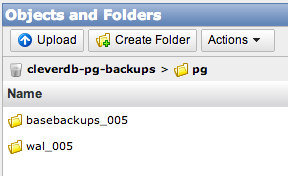
\includegraphics[width=0.6\textwidth]{wale1.pdf}}
  \caption{Папка бэкапов на S3}
  \label{fig:wal-e1}
\end{figure}

\begin{figure}[h!]
  \center{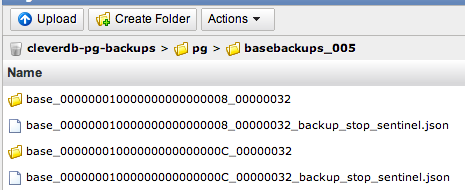
\includegraphics[width=0.6\textwidth]{wale2.pdf}}
  \caption{Папка бэкапов базы на S3}
  \label{fig:wal-e2}
\end{figure}

\begin{figure}[h!]
  \center{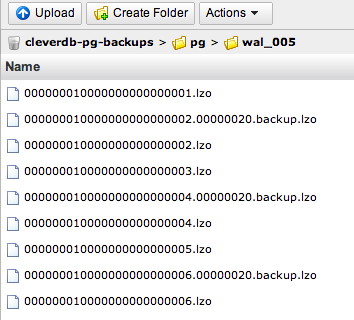
\includegraphics[width=0.6\textwidth]{wale3.pdf}}
  \caption{Папка WAL-логов на S3}
  \label{fig:wal-e3}
\end{figure}

Данный бэкап лучше делать раз в сутки (например, добавить в \lstinline!crontab!). На рис~\ref{fig:wal-e1}-\ref{fig:wal-e3} видно как хранятся бэкапы на S3. Все бэкапы сжаты через \href{http://en.wikipedia.org/wiki/Lzop}{lzop}. Данный алгоритм сжимает хуже чем gzip, но скорость сжатия намного быстрее (приблизительно 25 Мб/сек используя 5\% ЦПУ). Чтобы уменьшить нагрузку на чтение с жесткого диска бэкапы отправляются через \lstinline!pv! утилиту (опцией \lstinline!cluster-read-rate-limit! можно ограничить скорость чтения, если это требуется).

Теперь перейдем к восстановлению данных. Для восстановления базы из резервной копии используется \lstinline!backup-fetch! команда:

\begin{lstlisting}[language=Bash,label=lst:wal-e10,caption=Восстановление бэкапа базы из S3]
$ sudo -u postgres bash -c "envdir /etc/wal-e.d/env wal-e  --s3-prefix=s3://some-bucket/directory/or/whatever backup-fetch /var/lib/postgresql/9.2/main LATEST"
\end{lstlisting}

Где \lstinline!LATEST! означает, что база восстановится из последнего актуального бэкапа (PostgreSQL в это время должен быть остановлен). Для восстановления из более поздней резервной копии:

\begin{lstlisting}[language=Bash,label=lst:wal-e11,caption=Восстановление из поздней резервной копии]
$ sudo -u postgres bash -c "envdir /etc/wal-e.d/env wal-e  --s3-prefix=s3://some-bucket/directory/or/whatever backup-fetch /var/lib/postgresql/9.2/main base_LONGWALNUMBER_POSITION_NUMBER"
\end{lstlisting}

Для получения списка доступных резервных копий есть команда \lstinline!backup-list!:

\begin{lstlisting}[language=Bash,label=lst:wal-e12,caption=Список резервных копий]
$ envdir /etc/wal-e.d/env wal-e backup-list
name	last_modified	expanded_size_bytes	wal_segment_backup_start	wal_segment_offset_backup_start	wal_segment_backup_stop	wal_segment_offset_backup_stop
base_000000010000000000000008_00000032	2016-11-07T14:00:07.000Z		000000010000000000000008	00000032
base_00000001000000000000000C_00000032	2016-11-08T15:00:08.000Z		00000001000000000000000C	00000032
\end{lstlisting}

После завершения работы с основной резервной копией для полного восстановления нужно считать WAL-логи (чтобы данные обновились до последнего состояния). Для этого используется \lstinline!recovery.conf!:

\begin{lstlisting}[language=Bash,label=lst:wal-e13,caption=recovery.conf]
restore_command = 'envdir /etc/wal-e.d/env /usr/local/bin/wal-e wal-fetch "%f" "%p"'
\end{lstlisting}

После создания этого файла нужно запустить PostgreSQL. Через небольшой интервал времени база станет полностью восстановленной.

Для удаления старых резервных копий (или вообще всех) используется команда \lstinline!delete!:

\begin{lstlisting}[language=Bash,label=lst:wal-e14,caption=Удаление резервных копий]
# удаление старых бэкапов старше base_00000004000002DF000000A6_03626144
$ envdir /etc/wal-e.d/env wal-e delete --confirm before base_00000004000002DF000000A6_03626144
# удаление всех бэкапов
$ envdir /etc/wal-e.d/env wal-e delete --confirm everything
# удалить все старше последних 20 бэкапов
$ envdir /etc/wal-e.d/env wal-e delete --confirm retain 20
\end{lstlisting}

Без опции \lstinline!--confirm! команды будут запускаться и показывать, что будет удаляться, но фактического удаления не будет производиться (dry run).

\subsubsection{Заключение}

WAL-E помогает автоматизировать сбор резервных копий с PostgreSQL и хранить их в достаточно дешевом и надежном хранилище~--- Amazon S3 или Windows Azure.

\subsection{Barman}

\href{http://www.pgbarman.org/}{Barman}, как и WAL-E, позволяет создать систему для бэкапа и восстановления PostgreSQL на основе непрерывного резервного копирования. Barman использует для хранения бэкапов отдельный сервер, который может собирать бэкапы как с одного, так и с нескольких PostgreSQL баз данных.

\subsubsection{Установка и настройка}

Рассмотрим простой случай с одним экземпляром PostgreSQL (один сервер) и пусть его хост будет \lstinline!pghost!. Наша задача~--- автоматизировать сбор и хранение бэкапов этой базы на другом сервере (его хост будет \lstinline!brhost!). Для взаимодействия эти два сервера должны быть полностью открыты по SSH (доступ без пароля, по ключам). Для этого можно использовать \lstinline!authorized_keys! файл.

\begin{lstlisting}[language=Bash,label=lst:barman1,caption=Проверка подключения по SSH]
# Проверка подключения с сервера PostgreSQL (pghost)
$ ssh barman@brhost
# Проверка подключения с сервера бэкапов (brhost)
$ ssh postgres@pghost
\end{lstlisting}

Далее нужно установить на сервере для бэкапов barman. Сам barman написан на python и имеет пару зависимостей: python 2.6+, \lstinline!rsync! и python библиотеки (\lstinline!argh!, \lstinline!psycopg2!, \lstinline!python-dateutil!, \lstinline!distribute!). На Ubuntu все зависимости можно поставить одной командой:

\begin{lstlisting}[language=Bash,label=lst:barman2,caption=Установка зависимостей barman]
$ aptitude install python-dev python-argh python-psycopg2 python-dateutil rsync python-setuptools
\end{lstlisting}

Далее нужно установить barman:

\begin{lstlisting}[language=Bash,label=lst:barman3,caption=Установка barman]
$ tar -xzf barman-2.1.tar.gz
$ cd barman-2.1/
$ ./setup.py build
$ sudo ./setup.py install
\end{lstlisting}

Или используя \href{https://wiki.postgresql.org/wiki/Apt}{PostgreSQL Community APT репозиторий}:

\begin{lstlisting}[language=Bash,label=lst:barman-apt1,caption=Установка barman]
$ apt-get install barman
\end{lstlisting}

Теперь перейдем к серверу с PostgreSQL. Для того, чтобы barman мог подключаться к базе данных без проблем, нам нужно выставить настройки доступа в конфигах PostgreSQL:

\begin{lstlisting}[label=lst:barman4,caption=Отредактировать в postgresql.conf]
listen_adress = '*'
\end{lstlisting}

\begin{lstlisting}[label=lst:barman5,caption=Добавить в pg\_hba.conf]
host  all  all  brhost/32  trust
\end{lstlisting}

После этих изменений нужно перегрузить PostgreSQL. Теперь можем проверить с сервера бэкапов подключение к PostgreSQL:

\begin{lstlisting}[language=Bash,label=lst:barman6,caption=Проверка подключения к базе]
$ psql -c 'SELECT version()' -U postgres -h pghost
                                                  version
------------------------------------------------------------------------------------------------------------
 PostgreSQL 9.3.1 on x86_64-unknown-linux-gnu, compiled by gcc (Ubuntu/Linaro 4.7.2-2ubuntu1) 4.7.2, 64-bit
(1 row)
\end{lstlisting}

Далее создадим папку на сервере с бэкапами для хранения этих самых бэкапов:

\begin{lstlisting}[language=Bash,label=lst:barman7,caption=Папка для хранения бэкапов]
$ sudo mkdir -p /srv/barman
$ sudo chown barman:barman /srv/barman
\end{lstlisting}

Для настройки barman создадим \lstinline!/etc/barman.conf!:

\begin{lstlisting}[label=lst:barman8,caption=barman.conf]
[barman]
; Main directory
barman_home = /srv/barman

; Log location
log_file = /var/log/barman/barman.log

; Default compression level: possible values are None (default), bzip2, gzip or custom
compression = gzip

; 'main' PostgreSQL Server configuration
[main]
; Human readable description
description =  "Main PostgreSQL Database"

; SSH options
ssh_command = ssh postgres@pghost

; PostgreSQL connection string
conninfo = host=pghost user=postgres
\end{lstlisting}

Секция <<main>> (так мы назвали для barman наш PostgreSQL сервер) содержит настройки для подключения к PostgreSQL серверу и базе. Проверим настройки:

\begin{lstlisting}[language=Bash,label=lst:barman9,caption=Проверка barman настроек]
$ barman show-server main
Server main:
	active: true
	description: Main PostgreSQL Database
	ssh_command: ssh postgres@pghost
	conninfo: host=pghost user=postgres
	backup_directory: /srv/barman/main
	basebackups_directory: /srv/barman/main/base
	wals_directory: /srv/barman/main/wals
	incoming_wals_directory: /srv/barman/main/incoming
	lock_file: /srv/barman/main/main.lock
	compression: gzip
	custom_compression_filter: None
	custom_decompression_filter: None
	retention_policy: None
	wal_retention_policy: None
	pre_backup_script: None
	post_backup_script: None
	current_xlog: None
	last_shipped_wal: None
	archive_command: None
	server_txt_version: 9.3.1
	data_directory: /var/lib/postgresql/9.3/main
	archive_mode: off
	config_file: /etc/postgresql/9.3/main/postgresql.conf
	hba_file: /etc/postgresql/9.3/main/pg_hba.conf
	ident_file: /etc/postgresql/9.3/main/pg_ident.conf

# barman check main
Server main:
	ssh: OK
	PostgreSQL: OK
	archive_mode: FAILED (please set it to 'on')
	archive_command: FAILED (please set it accordingly to documentation)
	directories: OK
	compression settings: OK
\end{lstlisting}

Все хорошо, вот только PostgreSQL не настроен. Для этого на сервере с PostgreSQL отредактируем конфиг базы:

\begin{lstlisting}[label=lst:barman10,caption=Настройка PostgreSQL]
wal_level = hot_standby # archive для PostgreSQL < 9.0
archive_mode = on
archive_command = 'rsync -a %p barman@brhost:INCOMING_WALS_DIRECTORY/%f'
\end{lstlisting}

где \lstinline!INCOMING_WALS_DIRECTORY!~--- директория для складывания WAL-логов. Её можно узнать из вывода команды \lstinline!barman show-server main!(листинг~\ref{lst:barman9}, указано \lstinline!/srv/barman/main/incoming!). После изменения настроек нужно перегрузить PostgreSQL. Теперь проверим статус на сервере бэкапов:

\begin{lstlisting}[language=Bash,label=lst:barman11,caption=Проверка]
$ barman check main
Server main:
	ssh: OK
	PostgreSQL: OK
	archive_mode: OK
	archive_command: OK
	directories: OK
	compression settings: OK
\end{lstlisting}

Все готово. Для добавления нового сервера процедуру потребуется повторить, а в \lstinline!barman.conf! добавить новый сервер.


\subsubsection{Создание бэкапов}

Получение списка серверов:

\begin{lstlisting}[language=Bash,label=lst:barman12,caption=Список серверов]
$ barman list-server
main - Main PostgreSQL Database
\end{lstlisting}

Запуск создания резервной копии PostgreSQL (сервер указывается последним параметром):

\begin{lstlisting}[language=Bash,label=lst:barman13,caption=Создание бэкапа]
$ barman backup main
Starting backup for server main in /srv/barman/main/base/20121109T090806
Backup start at xlog location: 0/3000020 (000000010000000000000003, 00000020)
Copying files.
Copy done.
Asking PostgreSQL server to finalize the backup.
Backup end at xlog location: 0/30000D8 (000000010000000000000003, 000000D8)
Backup completed
\end{lstlisting}

Такую задачу лучше выполнять раз в сутки (добавить в cron). Посмотреть список бэкапов для указаной базы:

\begin{lstlisting}[language=Bash,label=lst:barman14,caption=Список бэкапов]
$ barman list-backup main
main 20121110T091608 - Fri Nov 10 09:20:58 2012 - Size: 1.0 GiB - WAL Size: 446.0 KiB
main 20121109T090806 - Fri Nov  9 09:08:10 2012 - Size: 23.0 MiB - WAL Size: 477.0 MiB
\end{lstlisting}

Более подробная информация о выбраной резервной копии:

\begin{lstlisting}[language=Bash,label=lst:barman15,caption=Информация о выбраной резервной копии]
$ barman show-backup main 20121110T091608
Backup 20121109T091608:
  Server Name       : main
  Status:           : DONE
  PostgreSQL Version: 90201
  PGDATA directory  : /var/lib/postgresql/9.3/main

  Base backup information:
    Disk usage      : 1.0 GiB
    Timeline        : 1
    Begin WAL       : 00000001000000000000008C
    End WAL         : 000000010000000000000092
    WAL number      : 7
    Begin time      : 2012-11-10 09:16:08.856884
    End time        : 2012-11-10 09:20:58.478531
    Begin Offset    : 32
    End Offset      : 3576096
    Begin XLOG      : 0/8C000020
    End XLOG        : 0/92369120

  WAL information:
    No of files     : 1
    Disk usage      : 446.0 KiB
    Last available  : 000000010000000000000093

  Catalog information:
    Previous Backup : 20121109T090806
    Next Backup     : - (this is the latest base backup)
\end{lstlisting}

Также можно сжимать WAL-логи, которые накапливаются в каталогах командой <<cron>>:

\begin{lstlisting}[language=Bash,label=lst:barman16,caption=Архивирование WAL-логов]
$ barman cron
Processing xlog segments for main
	000000010000000000000001
	000000010000000000000002
	000000010000000000000003
	000000010000000000000003.00000020.backup
	000000010000000000000004
	000000010000000000000005
	000000010000000000000006
\end{lstlisting}

Эту команду требуется добавлять в \lstinline!crontab!. Частота выполнения данной команды зависит от того, как много WAL-логов накапливается (чем больше файлов - тем дольше она выполняется). Barman может сжимать WAL-логи через gzip, bzip2 или другой компрессор данных (команды для сжатия и распаковки задаются через \lstinline!custom_compression_filter! и \lstinline!custom_decompression_filter! соответственно). Также можно активировать компрессию данных при передачи по сети через опцию \lstinline!network_compression! (по умолчанию отключена). Через опции \lstinline!bandwidth_limit! (по умолчанию 0, ограничений нет) и \lstinline!tablespace_bandwidth_limit! возможно ограничить использования сетевого канала.

Для восстановления базы из бэкапа используется команда \lstinline!recover!:

\begin{lstlisting}[language=Bash,label=lst:barman17,caption=Восстановление базы]
$ barman recover --remote-ssh-command "ssh postgres@pghost" main 20121109T090806 /var/lib/postgresql/9.3/main
Starting remote restore for server main using backup 20121109T090806
Destination directory: /var/lib/postgresql/9.3/main
Copying the base backup.
Copying required wal segments.
The archive_command was set to 'false' to prevent data losses.

Your PostgreSQL server has been successfully prepared for recovery!

Please review network and archive related settings in the PostgreSQL
configuration file before starting the just recovered instance.

WARNING: Before starting up the recovered PostgreSQL server,
please review also the settings of the following configuration
options as they might interfere with your current recovery attempt:

    data_directory = '/var/lib/postgresql/9.3/main'		# use data in another directory
    external_pid_file = '/var/run/postgresql/9.3-main.pid'		# write an extra PID file
    hba_file = '/etc/postgresql/9.3/main/pg_hba.conf'	# host-based authentication file
    ident_file = '/etc/postgresql/9.3/main/pg_ident.conf'	# ident configuration file
\end{lstlisting}

Barman может восстановить базу из резервной копии на удаленном сервере через SSH (для этого есть опция \lstinline!remote-ssh-command!). Также barman может восстановить базу, используя \href{http://en.wikipedia.org/wiki/Point-in-time\_recovery}{PITR}: для этого используются опции \lstinline!target-time! (указывается время) или \lstinline!target-xid! (id транзакции).


\subsubsection{Заключение}

Barman помогает автоматизировать сбор и хранение резервных копий PostgreSQL данных на отдельном сервере. Утилита проста, позволяет хранить и удобно управлять бэкапами нескольких PostgreSQL серверов.

\subsection{Pg\_arman}

\href{https://github.com/michaelpq/pg\_arman}{Pg\_arman}~--- менеджер резервного копирования и восстановления для PostgreSQL 9.5 или выше. Это ответвление проекта \lstinline!pg_arman!, изначально разрабатываемого в NTT. Теперь его разрабатывает и поддерживает Мишель Пакье. Утилита предоставляет следующие возможности:

\begin{itemize}
  \item Резервное копирование во время работы базы данных, включая табличные пространства, с помощью всего одной команды;
  \item Восстановление из резервной копии всего одной командой, с нестандартными вариантами, включая использование \href{https://www.postgresql.org/docs/current/static/continuous-archiving.html}{PITR};
  \item Поддержка полного и дифференциального копирования;
  \item Управление резервными копиями со встроенными каталогами;
\end{itemize}


\subsubsection{Использование}

Сначала требуется создать <<каталог резервного копирования>>, в котором будут храниться файлы копий и их метаданные. До инициализации этого каталога рекомендуется настроить параметры \lstinline!archive_mode! и \lstinline!archive_command! в \lstinline!postgresql.conf!. Если переменные инициализированы, \lstinline!pg_arman! может скорректировать файл конфигурации. В этом случае потребуется задать путь к кластеру баз данных: переменной окружения \lstinline!PGDATA! или через параметр \lstinline!-D/--pgdata!.

\begin{lstlisting}[language=Bash,label=lst:pgarman1,caption=init]
$ pg_arman init -B /path/to/backup/
\end{lstlisting}

После этого возможен один из следующих вариантов резервного копирования:

\begin{itemize}
  \item Полное резервное копирование (копируется весь кластер баз данных);
  \begin{lstlisting}[language=Bash,label=lst:pgarman2,caption=backup]
  $ pg_arman backup --backup-mode=full
  $ pg_arman validate
  \end{lstlisting}
  \item Дифференциальное резервное копирование: копируются только файлы или страницы, изменённые после последней проверенной копии. Для этого выполняется сканирование записей WAL от позиции последнего копирования до LSN выполнения \lstinline!pg_start_backup! и все изменённые блоки записываются и отслеживаются как часть резервной копии. Так как просканированные сегменты WAL должны находиться в архиве WAL, последний сегмент, задействованный после запуска \lstinline!pg_start_backup!, должен быть переключен принудительно;
  \begin{lstlisting}[language=Bash,label=lst:pgarman3,caption=backup]
  $ pg_arman backup --backup-mode=page
  $ pg_arman validate
  \end{lstlisting}
\end{itemize}

После резервного копирования рекомендуется проверять файлы копий как только это будет возможно. Непроверенные копии нельзя использовать в операциях восстановления и резервного копирования.

До начала восстановления через \lstinline!pg_arman! PostgreSQL кластер должен быть остановлен. Если кластер баз данных всё ещё существует, команда восстановления сохранит незаархивированный журнал транзакций и удалит все файлы баз данных. После восстановления файлов \lstinline!pg_arman! создаёт \lstinline!recovery.conf! в \lstinline!$PGDATA! каталоге. Этот конфигурационный файл содержит параметры для восстановления. После успешного восстановления рекомендуется при первой же возможности сделать полную резервную копию. Если ключ \lstinline!--recovery-target-timeline! не задан, целевой точкой восстановления будет \lstinline!TimeLineID! последней контрольной точки в файле (\lstinline!$PGDATA/global/pg_control!). Если файл \lstinline!pg_control! отсутствует, целевой точкой будет \lstinline!TimeLineID! в полной резервной копии, используемой при восстановлении.

\begin{lstlisting}[language=Bash,label=lst:pgarman4,caption=restore]
$ pg_ctl stop -m immediate
$ pg_arman restore
$ pg_ctl start
\end{lstlisting}

\lstinline!Pg_arman! имеет ряд ограничений:

\begin{itemize}
  \item Требуются права чтения каталога баз данных и записи в каталог резервного копирования. Обычно для этого на сервере БД требуется смонтировать диск, где размещён каталог резервных копий, используя NFS или другую технологию;
  \item Основные версии \lstinline!pg_arman! и сервера должны совпадать;
  \item Размеры блоков \lstinline!pg_arman! и сервера должны совпадать;
  \item Если в каталоге с журналами сервера или каталоге с архивом WAL оказываются нечитаемые файлы/каталоги, резервное копирование или восстановление завершится сбоем вне зависимости от выбранного режима копирования;
\end{itemize}


\section{Заключение}

В любом случае, усилия и время, затраченные на создание оптимальной системы создания бэкапов, будут оправданы. Невозможно предугадать когда произойдут проблемы с базой данных, поэтому бэкапы должны быть настроены для PostgreSQL (особенно, если это продакшн система).
